% Source: graduate-coursework/Prior_Semesters/Fa24/EMCH367/assignments/hw1/hw1.tex

\documentclass[border=4pt]{standalone}
\usepackage{amsmath}
\usepackage{amssymb}
\usepackage{graphicx}
\usepackage{tikz}
\usepackage{xcolor}

\begin{document}
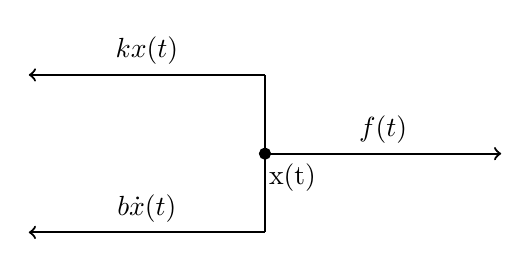
\begin{tikzpicture}
			      		    
		% Draw the point of interest
		\filldraw[black] (0,0) circle (2pt); % the point where forces are applied
			      		    
		% Draw the forces
		\draw[->, thick] (0,0) -- (3,0) node[midway, above] {$f(t)$}; % External force to the right
		\draw[<-, thick] (-3,1) -- (0,1) node[midway, above] {$kx(t)$}; % Spring force to the left
		\draw[<-, thick] (-3,-1) -- (0,-1) node[midway, above] {$b\dot{x}(t)$}; % Damping force to the left
		\draw (0,-1) -- (0,1);
			      		    
		% Add a label for the point
		\node[below] at (0.35,0) {x(t)};
			      		    
	\end{tikzpicture}
\end{document}
